\chapter{Results} \label{ch:result} During the training sessions, we have recorded five static gestures in 4 different positions in front of the robot. NAO is equipped with Asus Xtion and set in "Stand" posture. Head pitch of NAO is set to -18 degrees to look at the upper body of the user 1800 mm away from the sensor. First 3 positions of training are recorded at 1800 mm distance from the sensor in z axis and + /- 800 mm in x axis. Last training position is recorded at 2200 mm distance. Therefore, training data is recorded for 80 seconds of each gesture.

In this chapter, we present the results of real time hand gesture recognition for Human-robot interaction based on skeletal points tracking using depth camera. Training data for 5 classes with 11918 samples of 6 dimensional vector are trained with Adaptive Naive Bayes Classifier (ANBC). Min-Max scaling and Null Rejection with coefficient of 2.0 are enabled. Following sections illustrates the results of end-to-end interaction with robot using five gestures named as Walk, Turn Right, Turn Left, Move Right, Move Left gestures which are represented by the class labels 1,2,3,4,5 respectively.


\section{Gesture-To-Motion} 
\subsection{Walk} Figure \ref{res:gm:walk} shows that NAO is looking at the user to detect any possible gestures. When it recognized Walk gesture, Command module commands the robot to walk in forward direction for five seconds, thereby, completing a Gesture-To-Motion translation.

\begin{figure}
	[h] 
	\begin{minipage}
		{1 
		\textwidth} \centering 
		\includegraphics[height=85mm]{figures/result/usr-walk.jpg} \caption*{} 
	\end{minipage}
	\begin{minipage}
		{1 
		\textwidth} \hspace{-5 mm} 
		\includegraphics[width=160mm]{figures/result/nao-gm-walk.jpg} \caption*{} 
	\end{minipage}
	\caption{NAO recognizes Walk gesture and executes a predefined Gesture-To-Motion task.} \label{res:gm:walk} 
\end{figure}
\begin{figure}
	[h] \hspace{-15 mm} \centering 
	\includegraphics[width=155mm]{figures/result/test-walk.png} \caption{Our system is capable of real time prediction by processing 30 samples per second. However, the detected hand gesture is triggered only when it is gesticulated for 1 second because of the post-processing by Class Label Filter module. The graph shows 60 samples of correctly recognized Walk gesture. } \label{res:pl:walk} 
\end{figure}
\begin{figure}
	[h] \centering 
	\includegraphics[height=70mm]{figures/result/cc-walk.jpg} \caption{Control Center displays the recognized Walk gesture in real time with the positions of left and right hand in 3 dimensional space.} \label{res:cc:walk} 
\end{figure}


Figure \ref{res:pl:walk} shows the positions of left and right hand in x and y coordinates from the origin of the sensor. It is plotted using 60 input samples of Walk gesture. Figure \ref{res:cc:walk} shows the dashboard of Control Center that displays the prediction results. 

\clearpage 
\subsection{Turn Right} Figure \ref{res:gm:turn:right} shows that NAO received the input samples of left and right hand, and it recognized Turn Right gesture. The user commands NAO to turn at his right direction, thus, NAO turns at the mirrored direction (Left) for 5 seconds and stops to look for further gestures.

\begin{figure}
	[h] 
	\begin{minipage}
		{1 
		\textwidth} \centering 
		\includegraphics[height=75mm]{figures/result/usr-turn-right.png} \caption*{} 
	\end{minipage}
	\begin{minipage}
		{1 
		\textwidth} 
		\includegraphics[height=42mm]{figures/result/nao-gm-turn-right.png} 
	\end{minipage}
	\caption{Gesture-To-Motion Result of Turn Right} \label{res:gm:turn:right} 
\end{figure}
\begin{figure}
	[h] \centering 
	\includegraphics[height=110mm]{figures/result/test-turn-right.png} \caption{60 samples (2 Seconds) of correctly recognized Turn Right gesture}
	\label{res:pl:turn:right} 
\end{figure}
\begin{figure}
	[h] \centering 
	\includegraphics[height=70mm]{figures/result/cc-turn-right.png} \caption{Control Center is showing the prediction results of Turn Right gesture} 
	\label{res:cc:turn:right}	
\end{figure}

Figure \ref{res:pl:turn:right} shows the positions of left and right hand in x and y coordinates from the origin of the sensor. It is plotted using 60 input samples of Turn Right gesture. Figure \ref{res:cc:turn:right} shows the dashboard of Control Center that displays the prediction results. 

\clearpage 
\subsection{Turn Left} Figure \ref{res:gm:turn:left} shows that NAO received the input samples of left and right hand, and it recognized Turn Left gesture. The user commands NAO to turn at his left direction, thus, NAO turns at the mirrored direction (Right) for 5 seconds and stops to look for further gestures.

\begin{figure}
	[h] 
	\begin{minipage}
		{1 
		\textwidth} \centering 
		\includegraphics[height=75mm]{figures/result/usr-turn-left.jpg} \caption*{} 
	\end{minipage}
	\begin{minipage}
		{1 
		\textwidth} 
		\includegraphics[height=42mm]{figures/result/nao-gm-turn-left.jpg} 
	\end{minipage}
	\caption{Gesture-To-Motion Result of Turn Left} \label{res:gm:turn:left} 
\end{figure}

\begin{figure}
	[h] \centering 
	\includegraphics[height=110mm]{figures/result/test-turn-left.jpg} \caption{60 samples (2 Seconds) of correctly recognized Turn Left gesture} 
	\label{res:pl:turn:left}
\end{figure}

\begin{figure}
	[h] \centering 
	\includegraphics[height=70mm]{figures/result/cc-turn-left.jpg} \caption{Control Center is showing the prediction results of Turn Left gesture}
	\label{res:cc:turn:left} 
\end{figure}


Figure \ref{res:pl:turn:left} shows the positions of left and right hand in x and y coordinates from the origin of the sensor. It is plotted using 60 input samples of Turn Left gesture. Figure \ref{res:cc:turn:left} shows the dashboard of Control Center that displays the prediction results. 

\clearpage 
\subsection{Move Right} Figure \ref{res:gm:move:right} shows that NAO recognizes Move Right gesture as soon as the user gesticulated it using both the tracked hands. Like other gestures, this is also perceived by NAO to move in the mirrored direction of the user. Hence, NAO turns left for 3 seconds and move in forward direction for 5 seconds.

\begin{figure}
	[h] 
	\begin{minipage}
		{1 
		\textwidth} \centering 
		\includegraphics[height=75mm]{figures/result/usr-move-right.png} \caption*{} 
	\end{minipage}
	\begin{minipage}
		{1 
		\textwidth} 
		\includegraphics[height=42mm]{figures/result/nao-gm-move-right.png} 
	\end{minipage}
	\caption{Gesture-To-Motion Result of Move Right} \label{res:gm:move:right} 
\end{figure}
\begin{figure}
	[h] \centering 
	\includegraphics[height=110mm]{figures/result/test-move-right.png} \caption{60 samples (2 Seconds) of correctly recognized Move Right gesture}
	\label{res:pl:move:right}  
\end{figure}
\begin{figure}
	[h] \centering 
	\includegraphics[height=70mm]{figures/result/cc-move-right.png} \caption{Control Center is showing the prediction results of Move Right gesture}
	\label{res:cc:move:right} 
\end{figure}


Figure \ref{res:pl:move:right} shows the positions of left and right hand in x and y coordinates from the origin of the sensor. It is plotted using 60 input samples of Move Right gesture. Figure \ref{res:cc:move:right} shows the dashboard of Control Center that displays the prediction results. 

\clearpage 
\subsection{Move Left} Figure \ref{res:gm:move:left} shows that NAO recognizes Move Left gesture as soon as the user gesticulated it using both the tracked hands. Like other gestures, this is also perceived by NAO to move in the mirrored direction of the user. Hence, NAO turns right for 3 seconds and move in forward direction for 5 seconds.

\begin{figure}
	[h] 
	\begin{minipage}
		{1 
		\textwidth} \centering 
		\includegraphics[height=75mm]{figures/result/usr-move-left.jpg} \caption*{} 
	\end{minipage}
	\begin{minipage}
		{1 
		\textwidth} 
		\includegraphics[height=42mm]{figures/result/nao-gm-move-left.jpg} 
	\end{minipage}
	\caption{Gesture-To-Motion Result of Move Left} \label{res:gm:move:left} 
\end{figure}
\begin{figure}
	[h] \centering 
	\includegraphics[height=110mm]{figures/result/test-move-left.jpg} \caption{60 samples (2 Seconds) of correctly recognized Move Left gesture}
	\label{res:pl:move:left}	 
\end{figure}
\begin{figure}
	[h] \centering 
	\includegraphics[height=70mm]{figures/result/cc-move-left.jpg} \caption{Control Center is showing the prediction results of Move Left gesture}
	\label{res:cc:move:left}	 
\end{figure}


Figure \ref{res:pl:move:left} shows the positions of left and right hand in x and y coordinates from the origin of the sensor. It is plotted using 60 input samples of Move Left gesture. Figure \ref{res:cc:move:left} shows the dashboard of Control Center that displays the prediction results. 

\clearpage

\section{Gesture-To-Gesture} Figure \ref{res:gg} shows how human hand gestures are translated to robotic hand gestures. When a gesture is detected, the Command module sets the predefined angles to the shoulder and elbow joints of both the hands of NAO to perform Gesture-To-Gesture translation. 

\begin{figure}
	[h]	 	
	\begin{minipage}
		{.3 
			\textwidth}  		
		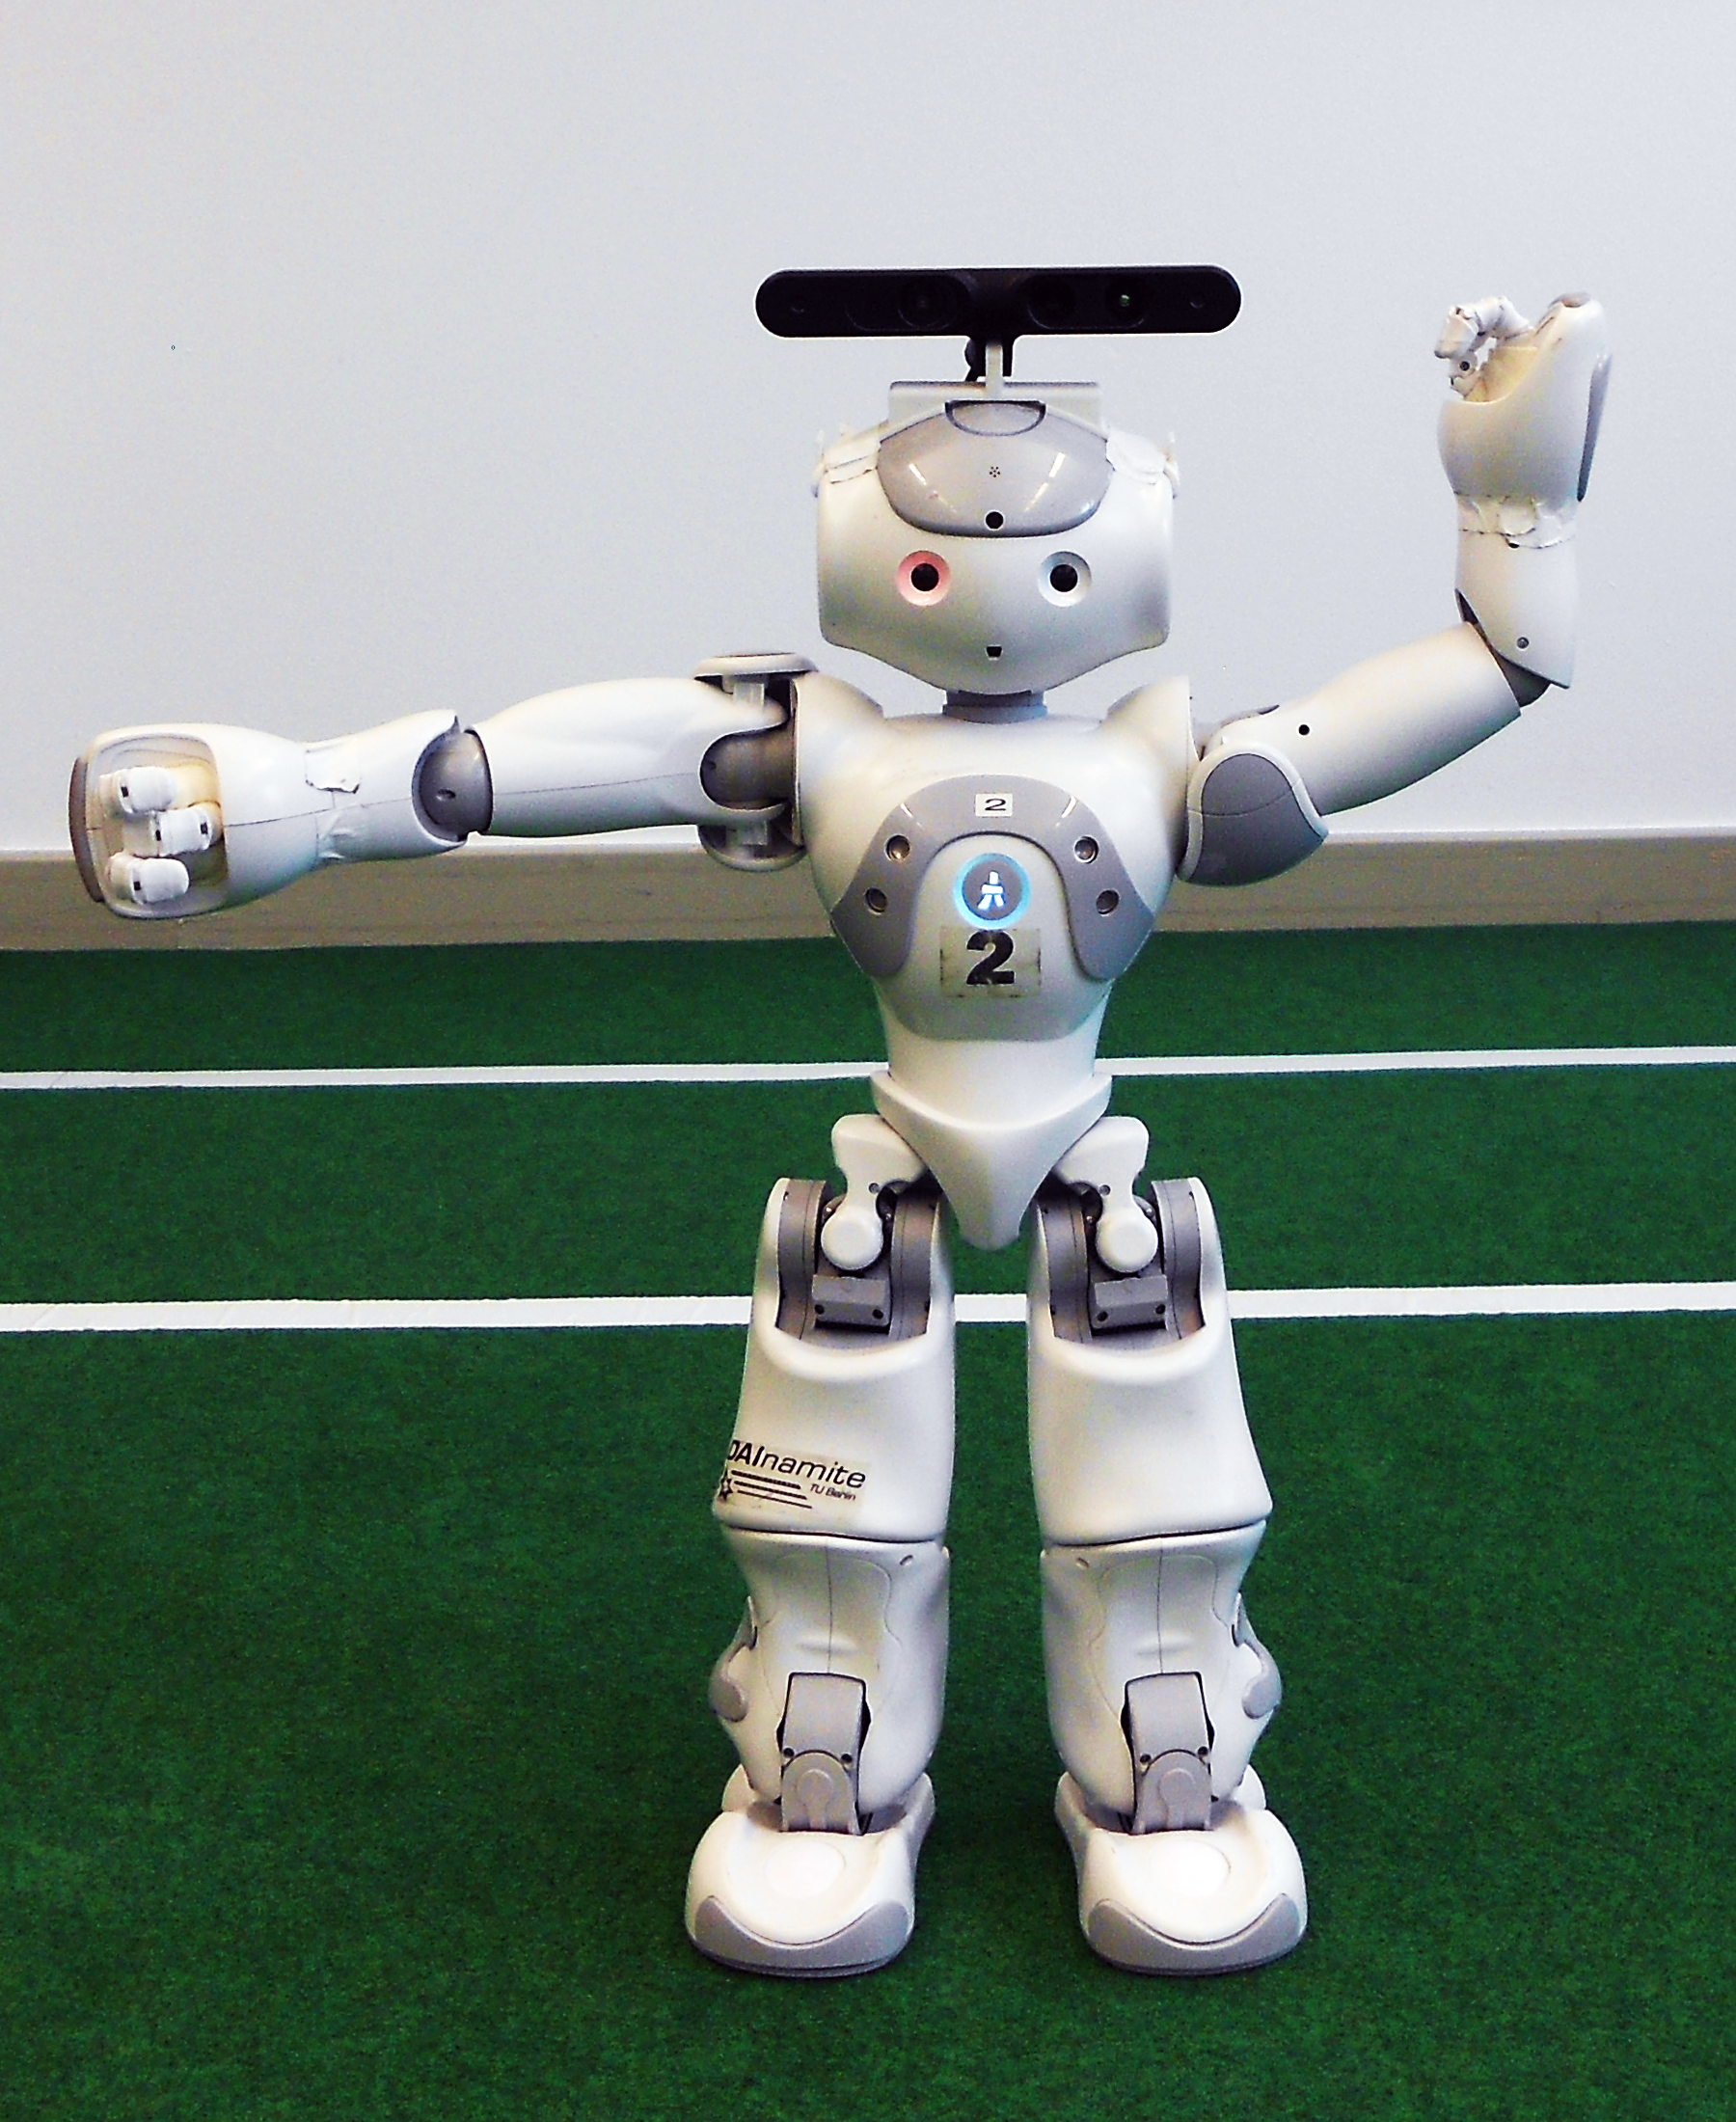
\includegraphics[height=55mm]{figures/result/nao-gg-turn-right.png} \caption*{Turn Right } 
	\end{minipage}
	\begin{minipage}
		{.3 
			\textwidth}  
		
		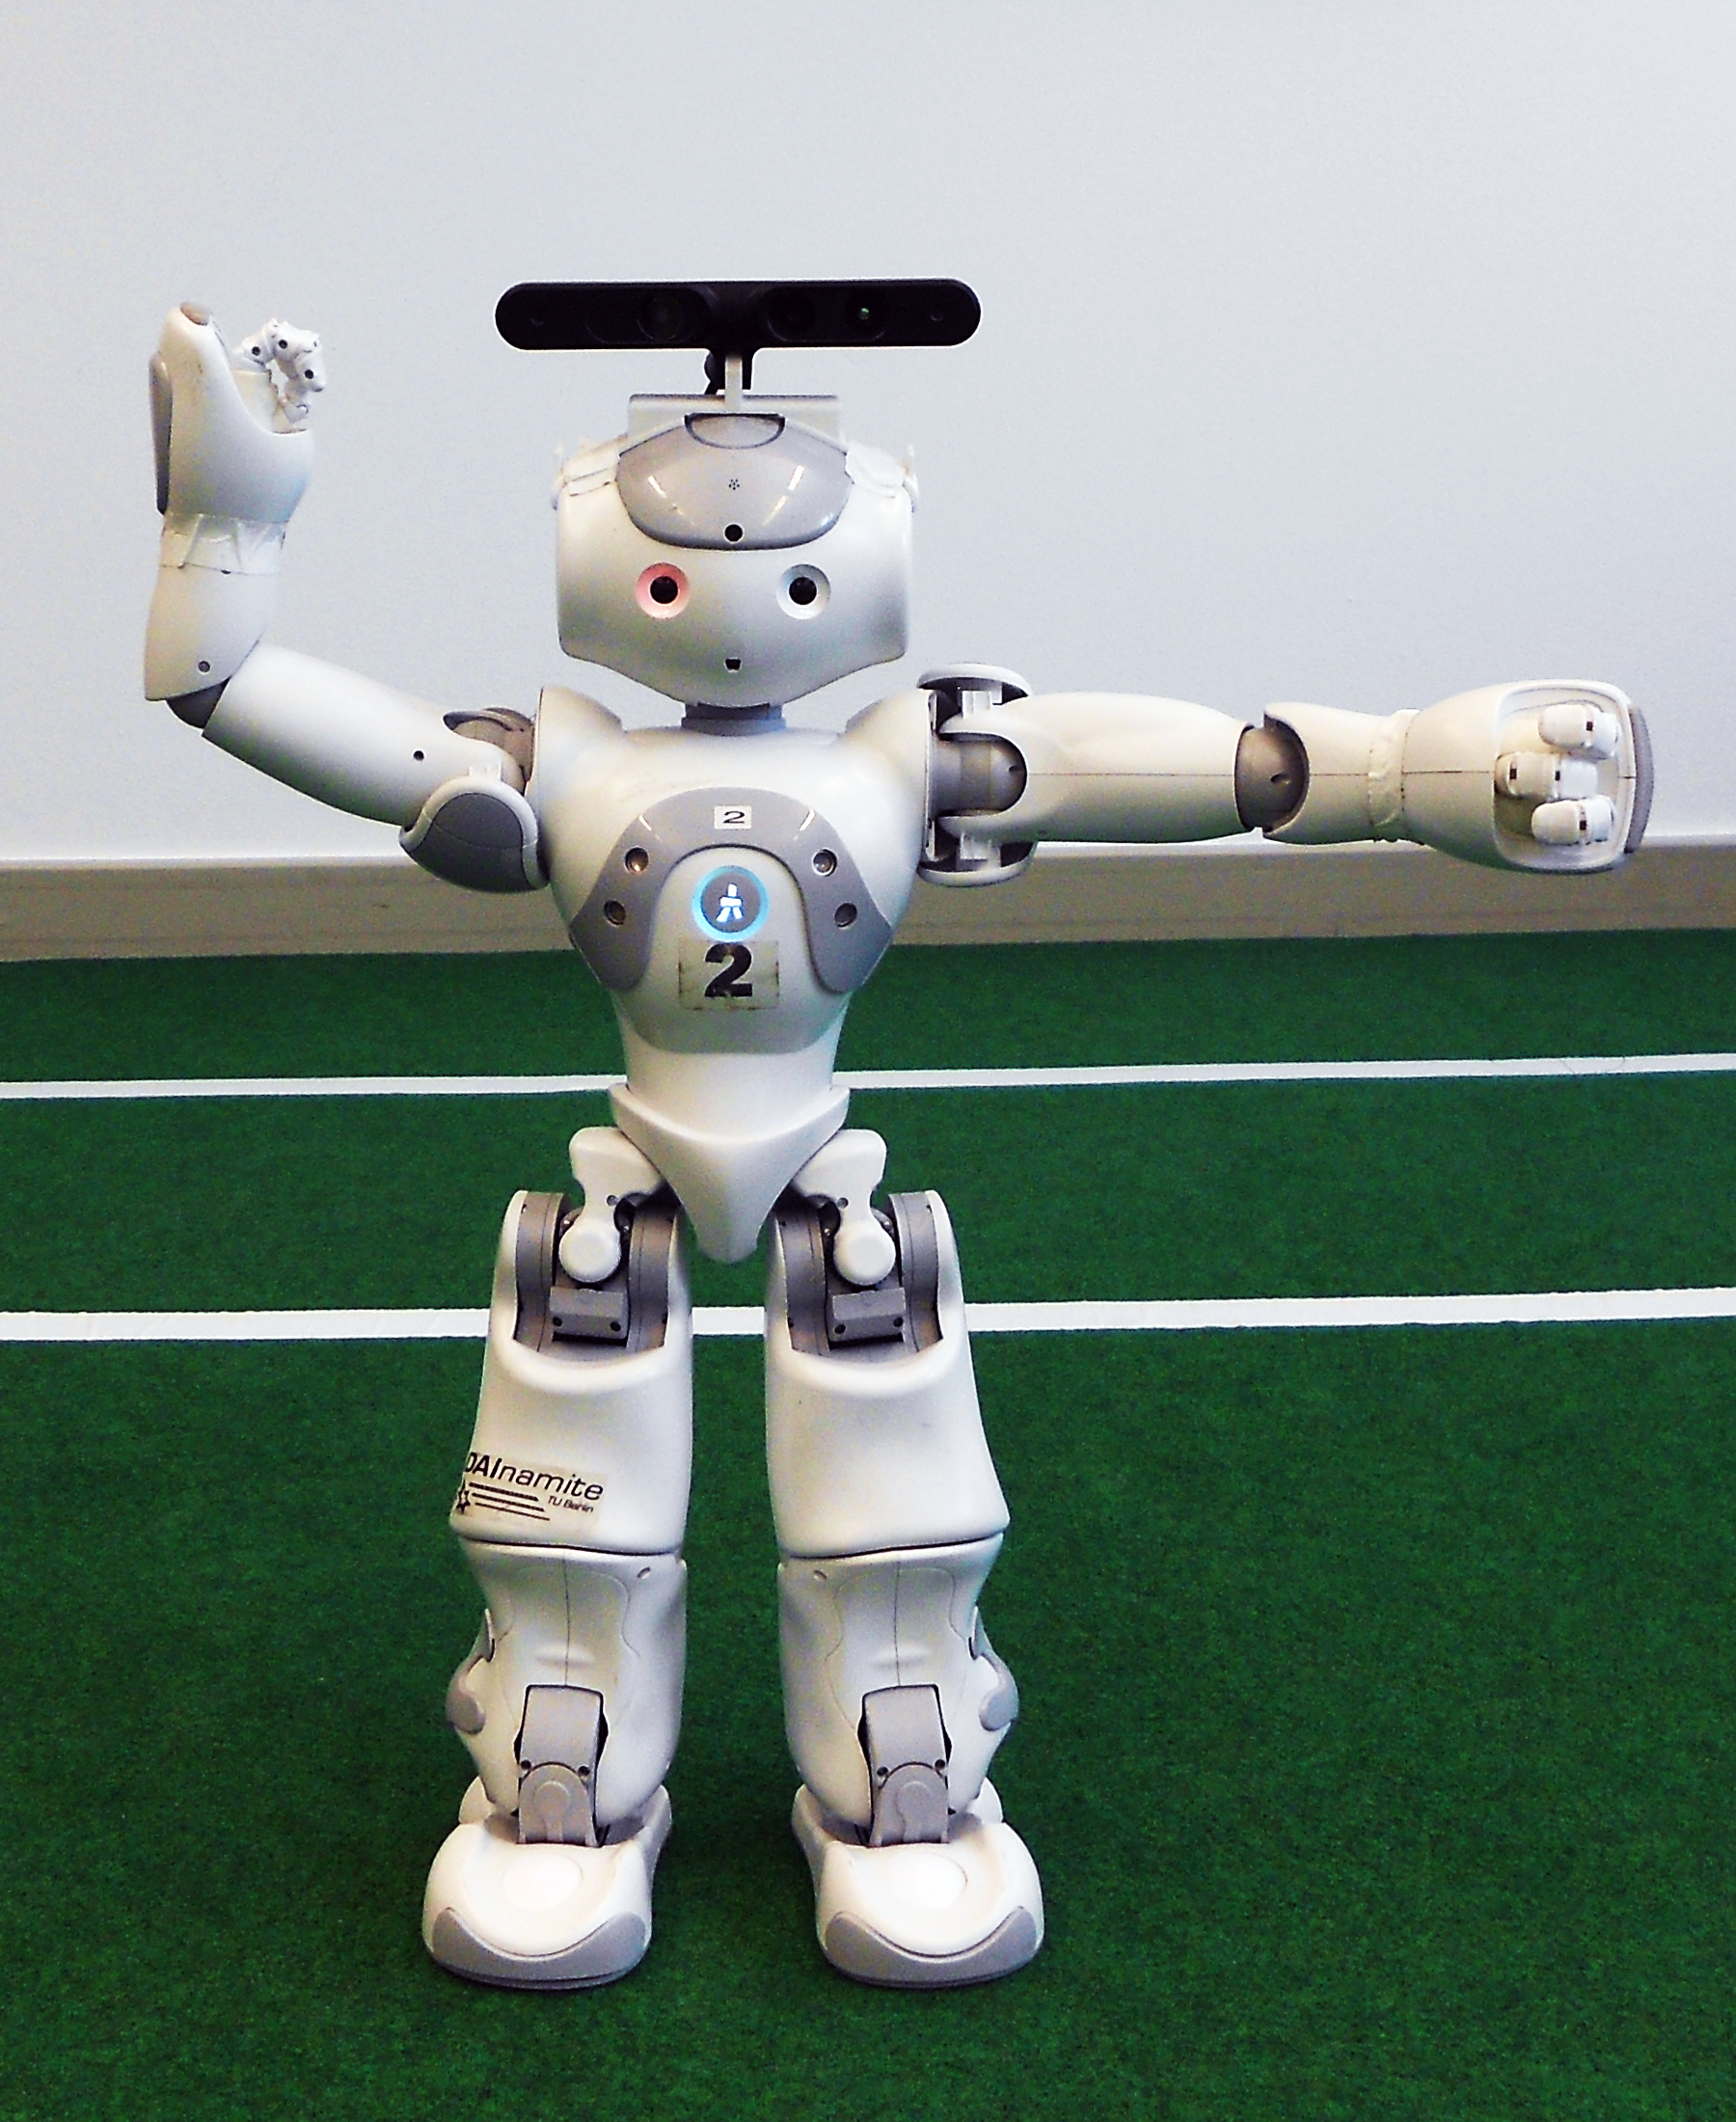
\includegraphics[height=55mm]{figures/result/nao-gg-turn-left.png} \caption*{Turn Left }
	\end{minipage}
	\begin{minipage}
		{.3
			\textwidth}  
		
		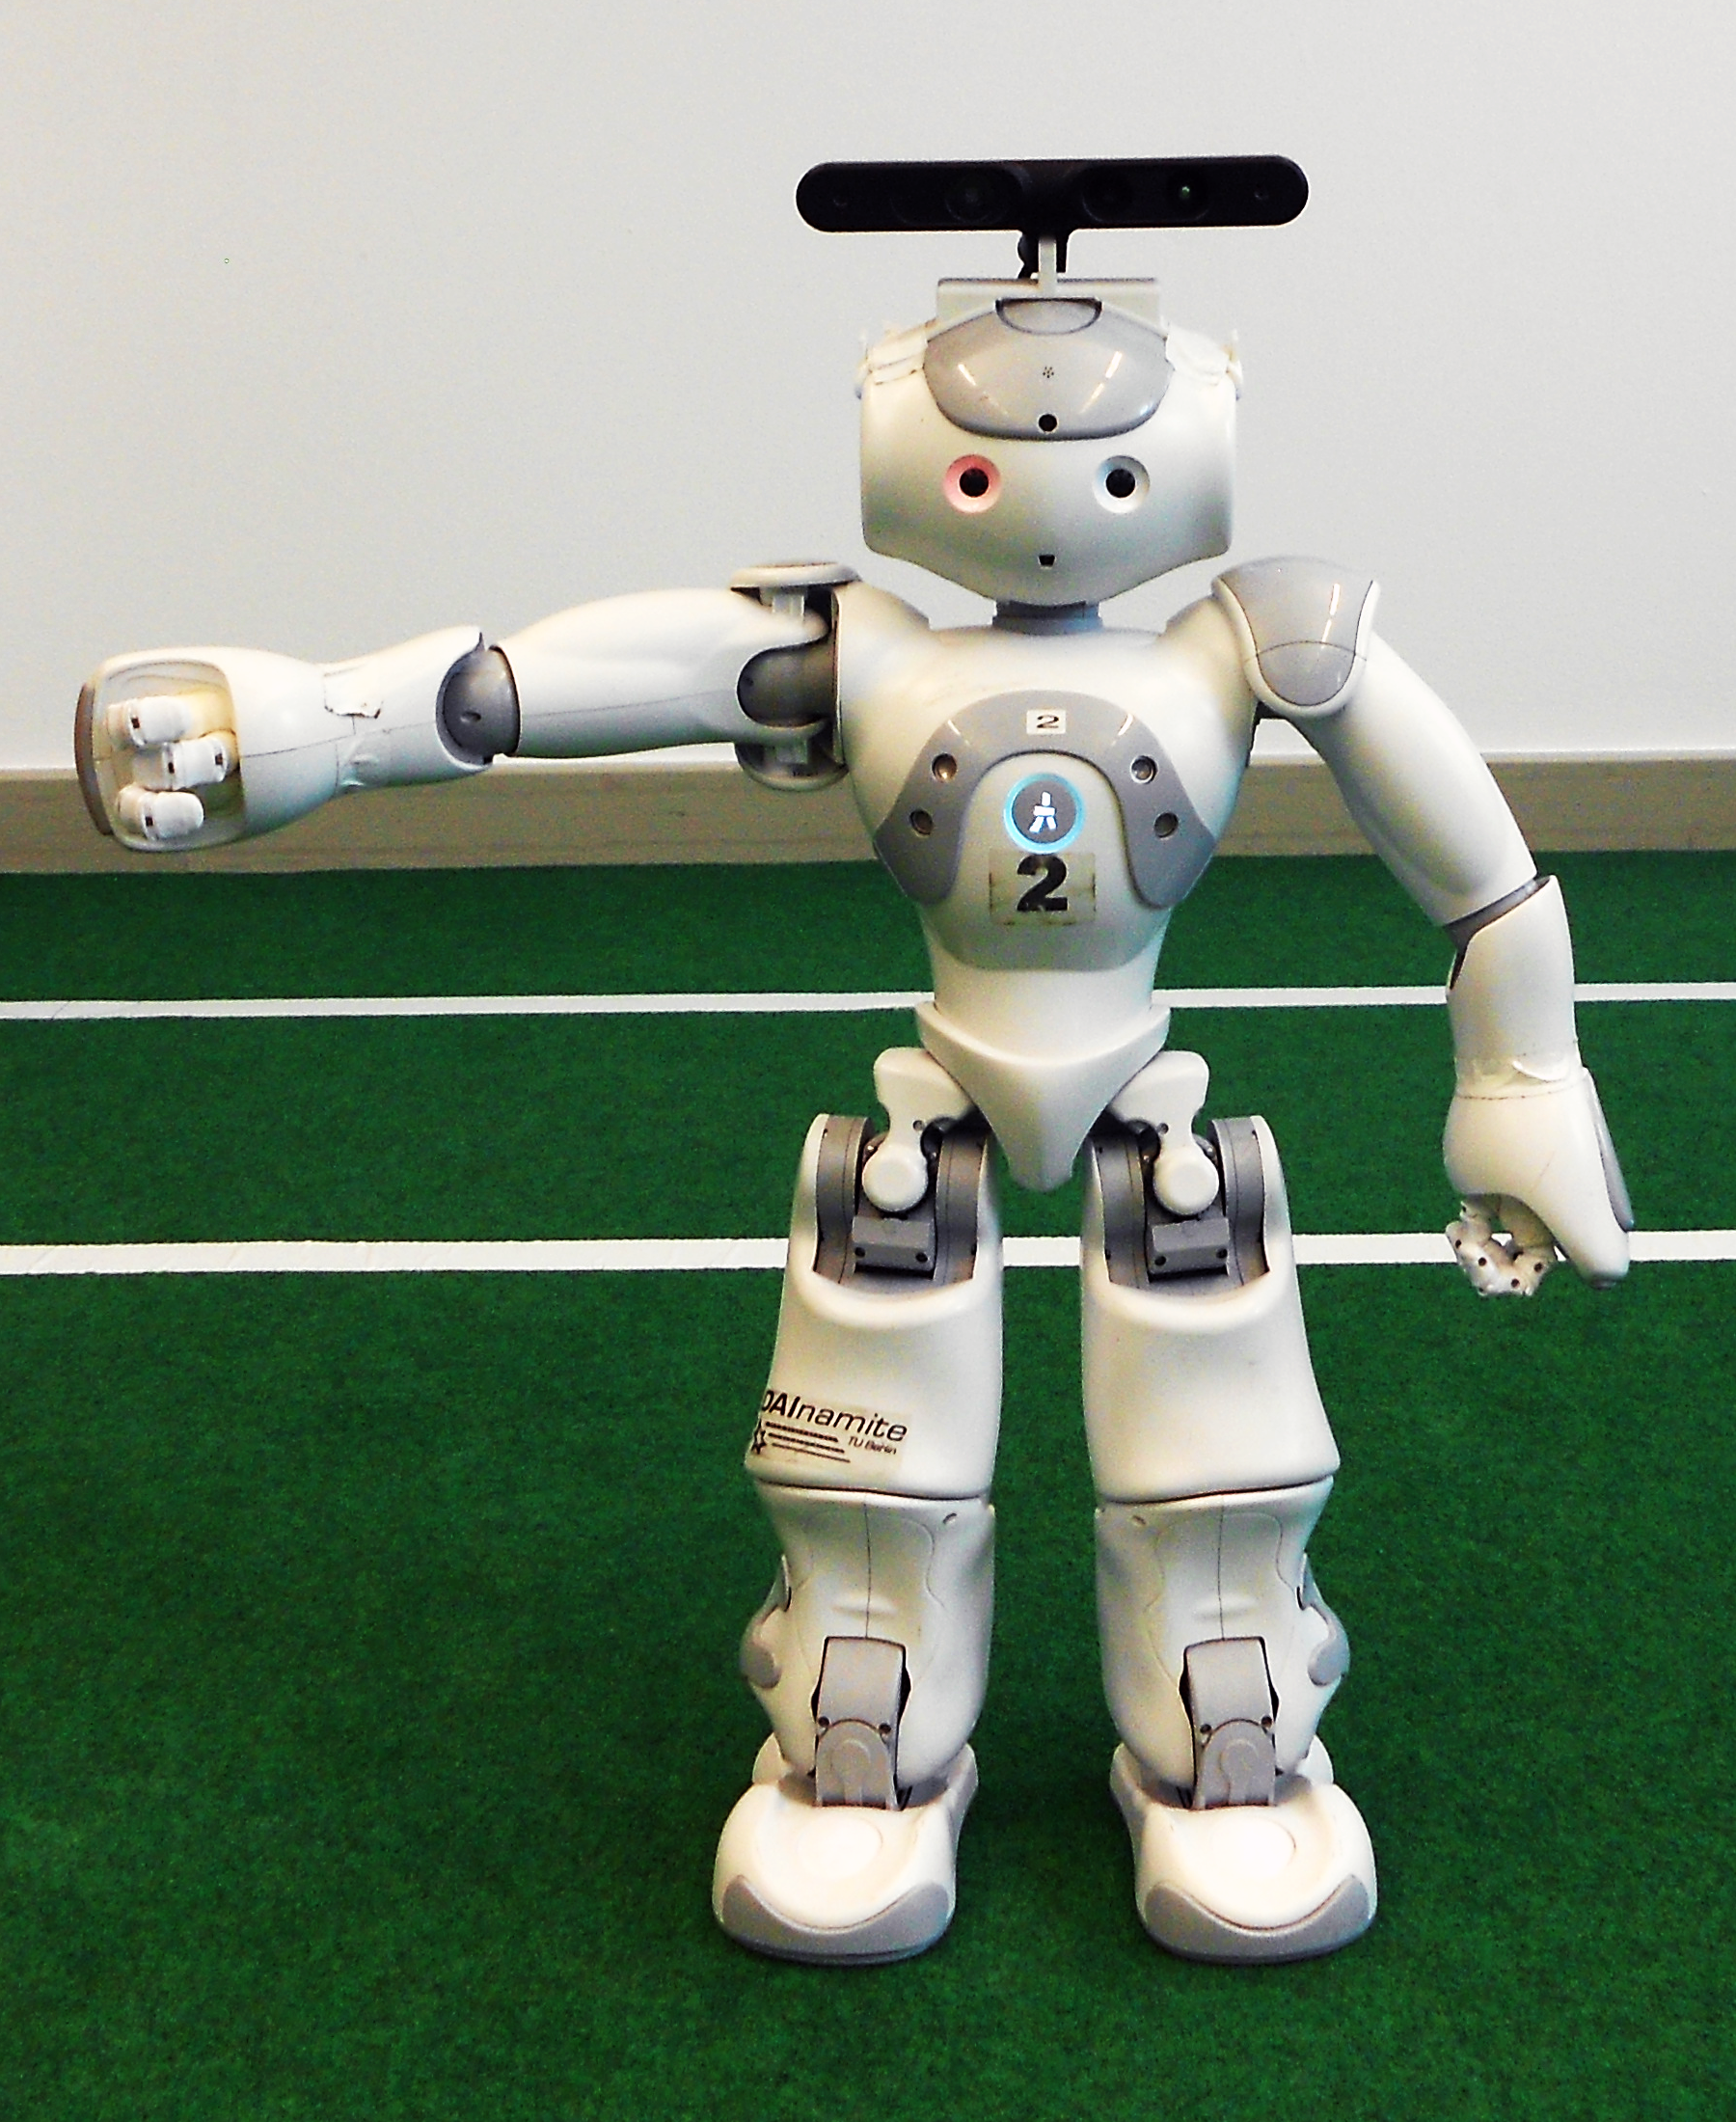
\includegraphics[height=55mm]{figures/result/nao-gg-move-right.png} \caption*{Move Right}
	\end{minipage}
	\begin{minipage}
		{.3
			\textwidth}  
		
		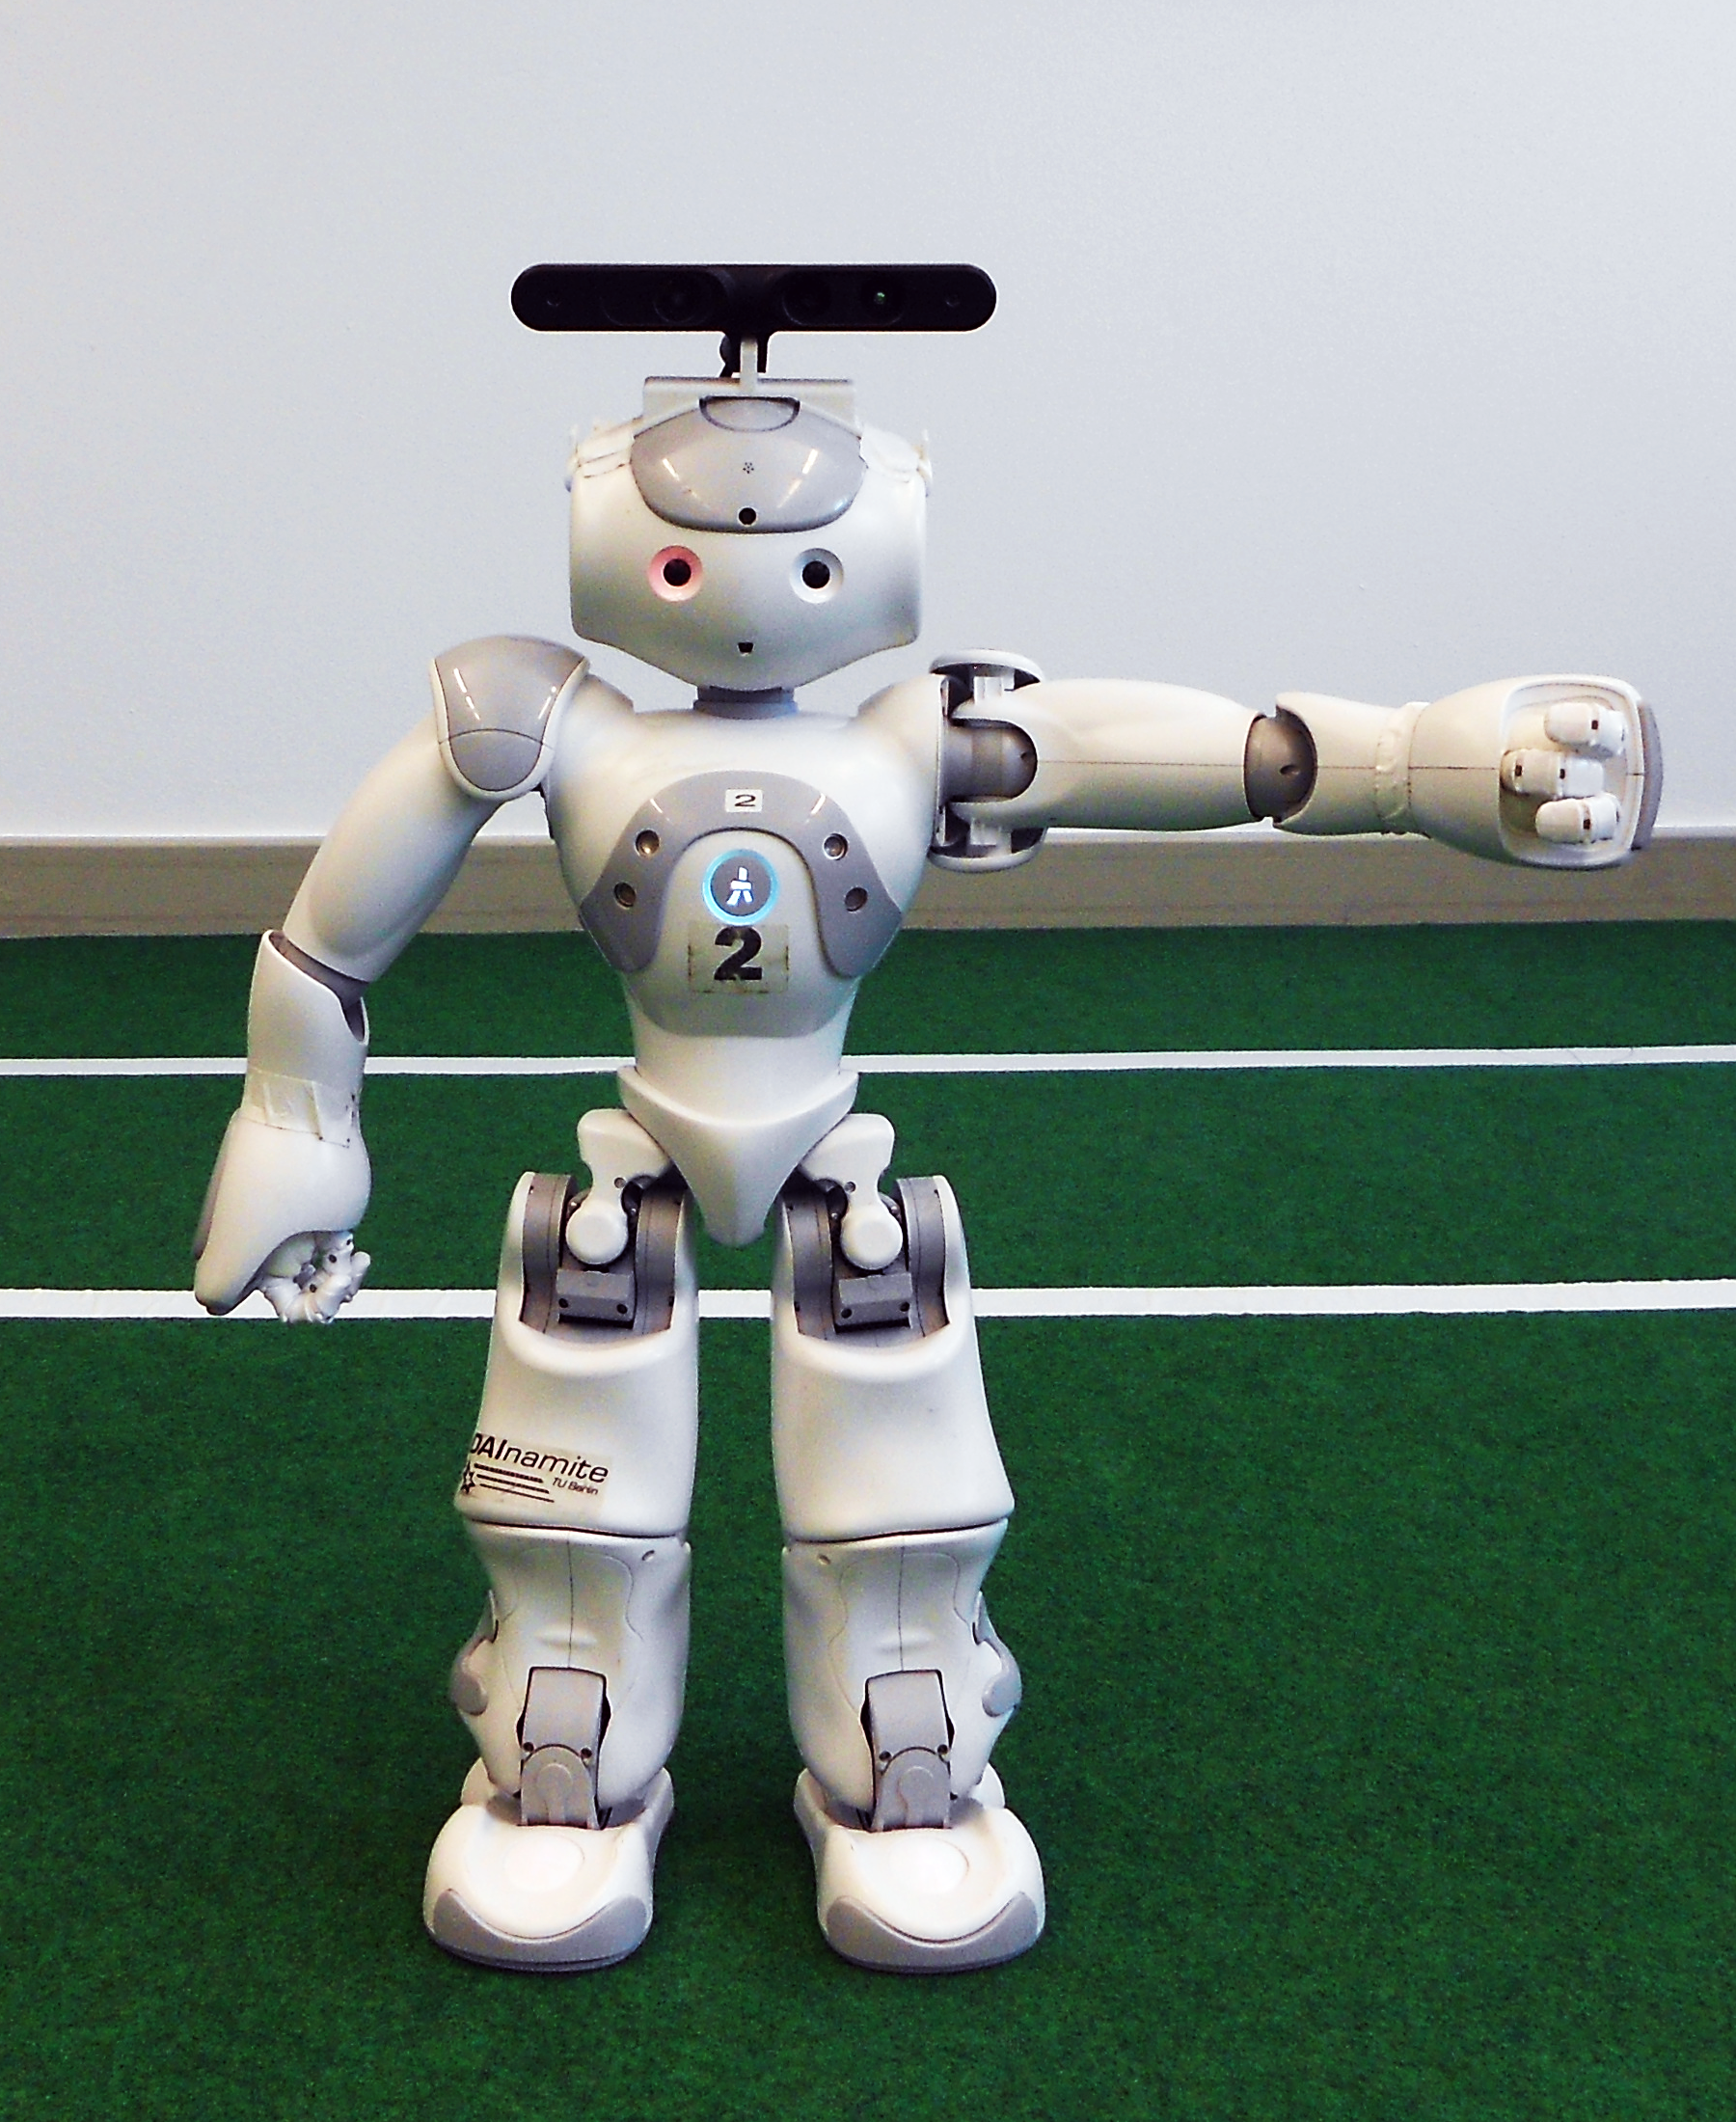
\includegraphics[height=55mm]{figures/result/nao-gg-move-left.png} \caption*{Move Left}
	\end{minipage}
	\begin{minipage}
		{.4
			\textwidth}  
		\centering
		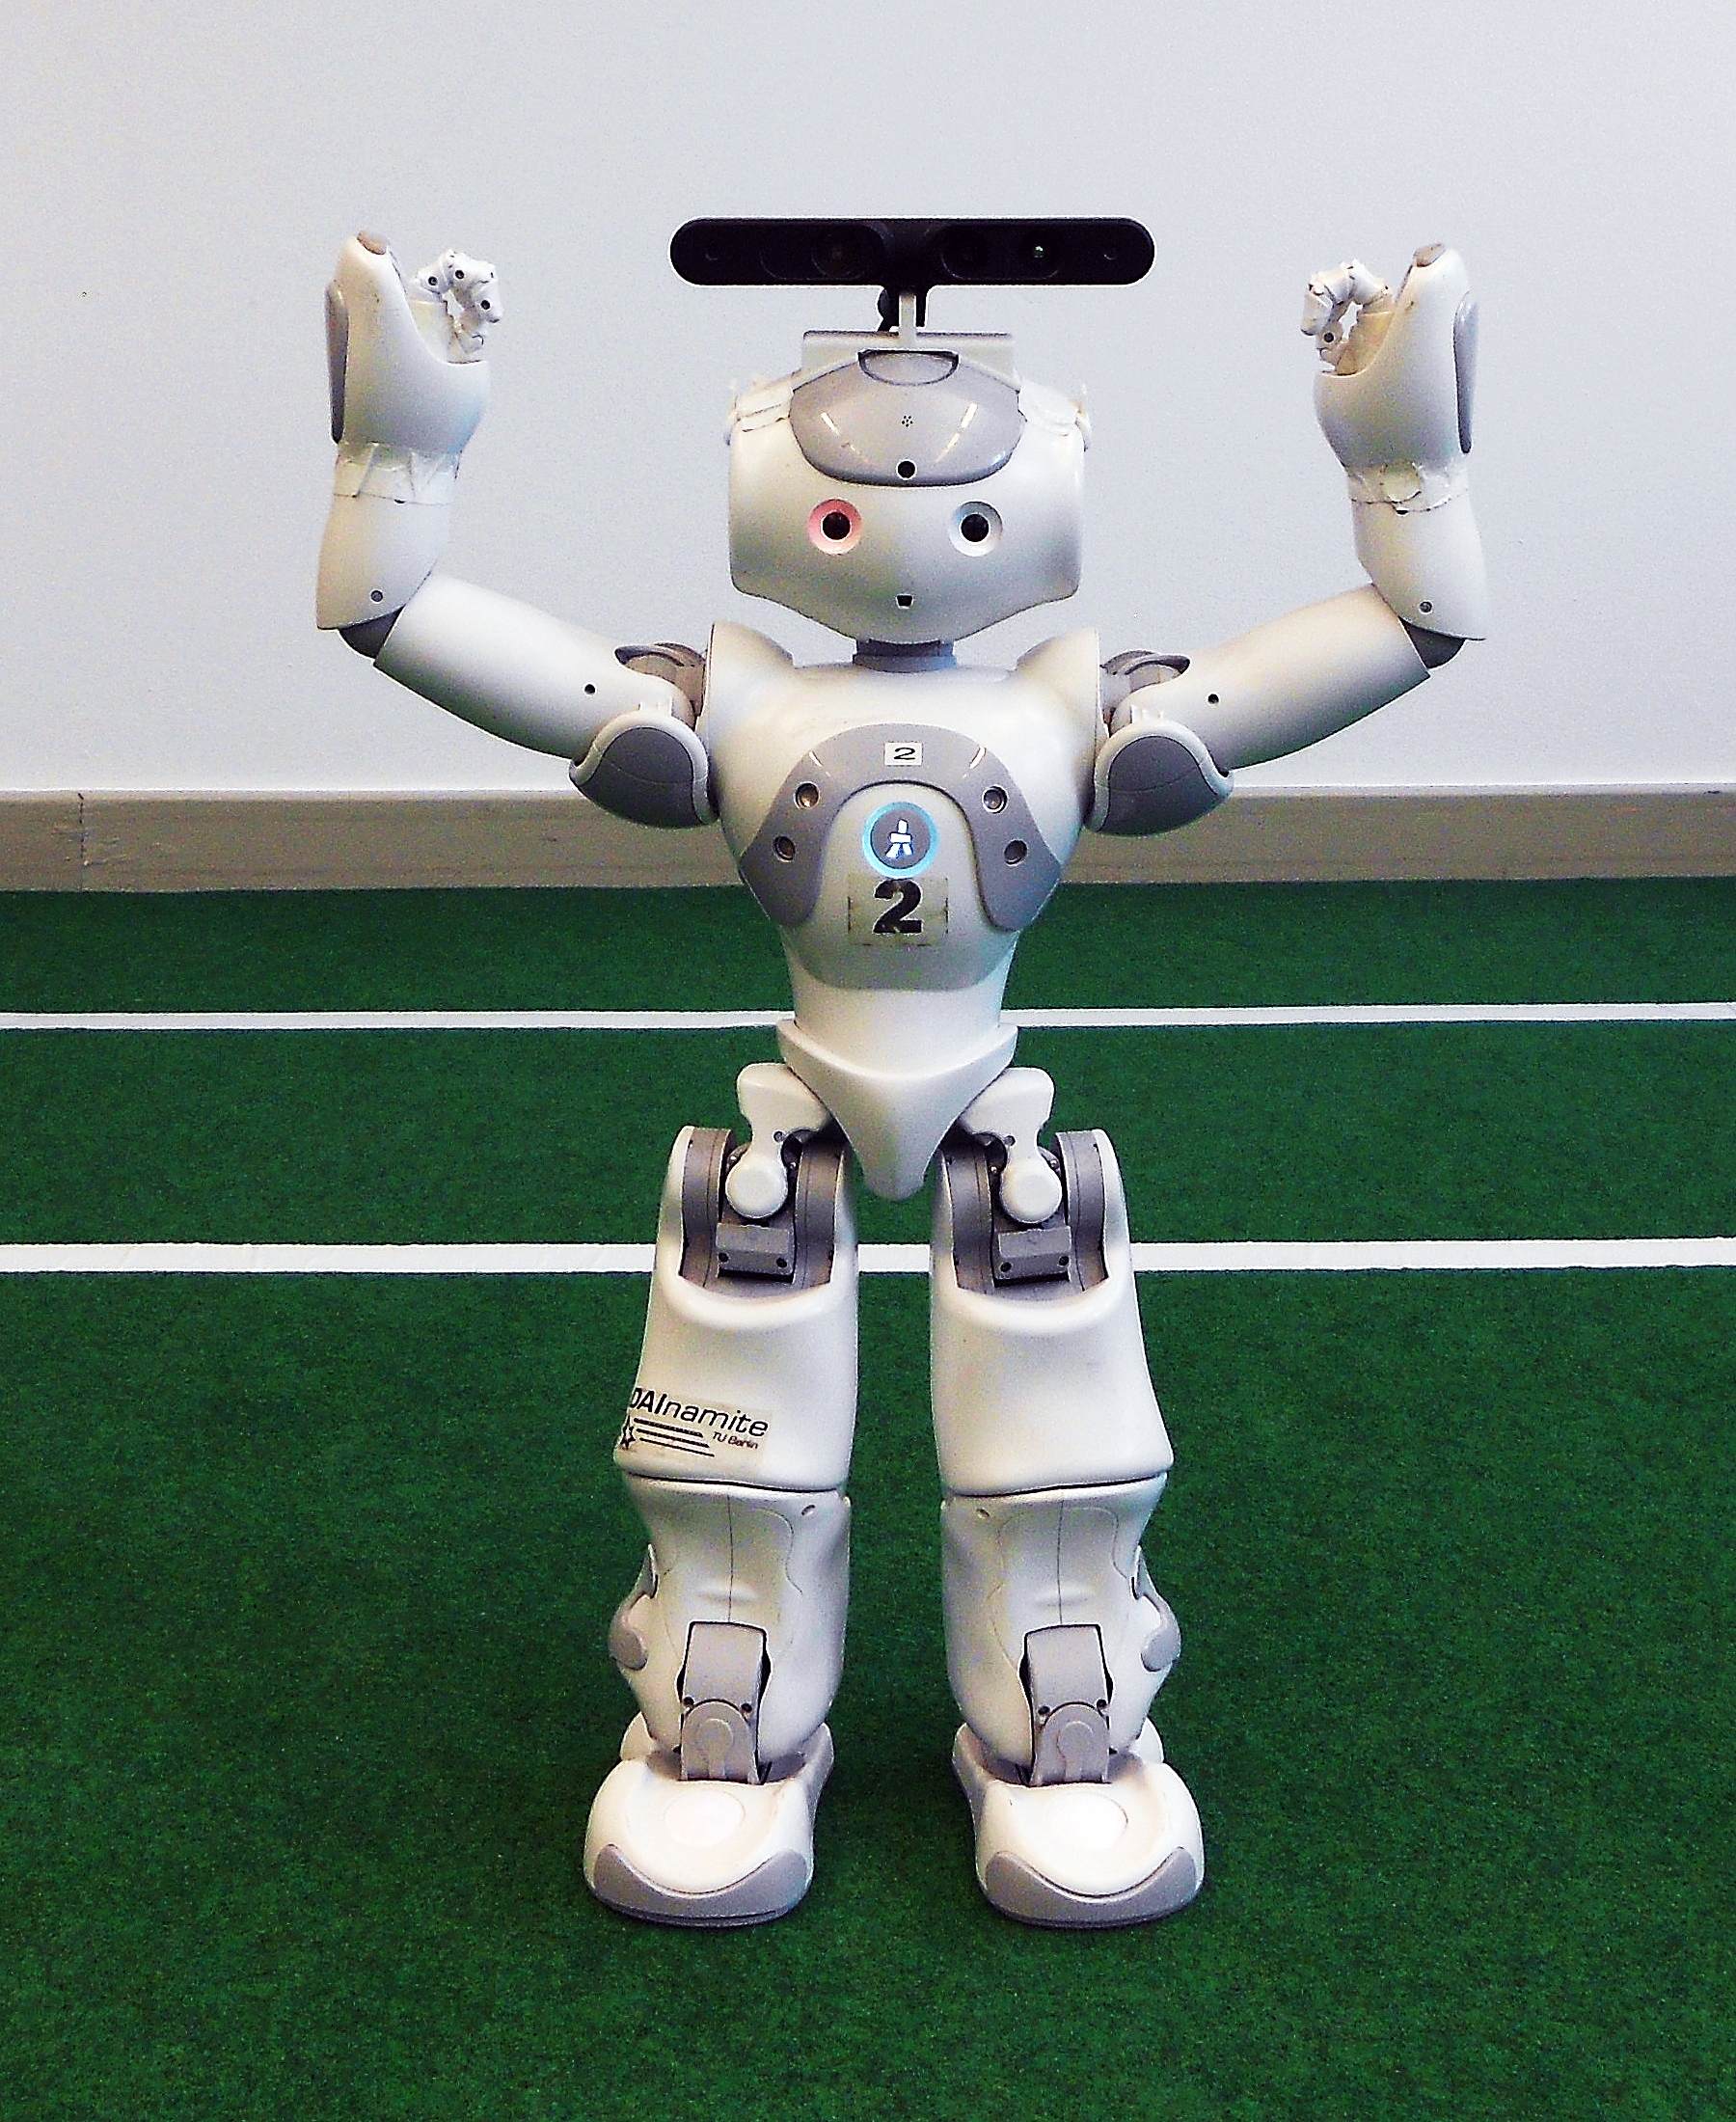
\includegraphics[height=55mm]{figures/result/nao-gg-walk.png} 
		\caption*{Walk}
	\end{minipage}	
	\caption{Results of Gesture-To-Gesture translation}
	\label{res:gg}
\end{figure}


\section{Evaluation} In this section, we present the experiments carried out to evaluate and validate our system to recognize hand gestures using skeletal points. The goal is to demonstrate the effectiveness of the classifier and to evaluate its potential for real time prediction. In the classification phase, input samples are normalized using Min-Max Scaling and Null Rejection is enabled to detect non-gestures. Therefore, the evaluation demonstrates the prediction accuracy of ANBC with various null rejection coefficient and the comparison it with other supervised learning classifier such as Minimum Distance (MinDist).

\begin{table}
	\centering
	\pgfplotstabletypeset [ col sep=comma, every head row/.style={before row=\hline,after row=\hline}, every last row/.style={after row=\hline}, ] {../../data/results/mean.csv}
	\caption{Normalized mean values of 3 dimensions of left and right hand} \label{tb:ev:mean} 
\end{table}

\begin{table}
	\centering
	\pgfkeys{/pgf/number format/.cd,fixed,fixed zerofill,precision=3}
	\pgfplotstabletypeset [ col sep=comma, every head row/.style={before row=\hline,after row=\hline}, every last row/.style={after row=\hline}, ] {../../data/results/sd.csv} \caption{Standard deviations of 3 dimensions of left and right hand} \label{tb:ev:sd} 
\end{table}

\begin{table}
	\centering
		\pgfkeys{/pgf/number format/.cd,fixed,fixed zerofill,precision=3}
	\pgfplotstabletypeset [ 
	col sep=comma, 
	every head row/.style={before row=\hline,after row=\hline},
	every last row/.style={after row=\hline},
	create on use/newcol/.style={
		create col/set list={Precision,Recall,F-measure}
	},
	columns/newcol/.style={string type},
	columns={newcol,0,1,2,3,4},
	display columns/0/.style={column name={}},
	display columns/1/.style={column name={Class 1}},
	display columns/2/.style={column name={Class 2}},
	display columns/3/.style={column name={Class 3}},
	display columns/4/.style={column name={Class 4}},
	display columns/5/.style={column name={Class 5}},
	] 
	{../../data/results/subset-test/anbc2-precision-recall-fmeasure.csv}
	\caption{Precision, Recall and F-Measure calculated by validating 10\% of training dataset. ANBC Classifier trained with Null Rejection coefficient 2.0} \label{tb:ev:confusion} 
\end{table}


\begin{table}
	\centering
	\pgfkeys{/pgf/number format/.cd,fixed,fixed zerofill,precision=3}
	\pgfplotstabletypeset [ 
	col sep=comma, 
	every head row/.style={before row=\hline,after row=\hline},
	every last row/.style={after row=\hline},
	create on use/newcol/.style={
		create col/set list={Non-gesture,Class 1,Class 2,Class 3,Class 4,Class 5}
	},
	columns/newcol/.style={string type},
	columns={newcol,0,1,2,3,4,5},
	display columns/0/.style={column name={}},
	display columns/1/.style={column name={Non-Gesture}},
	display columns/2/.style={column name={Class 1}},
	display columns/3/.style={column name={Class 2}},
	display columns/4/.style={column name={Class 3}},
	display columns/5/.style={column name={Class 4}},
	display columns/6/.style={column name={Class 5}},				
	] 
	{../../data/results/subset-test/anbc2-confusion.csv}
	\caption{Confusion Matrix calculated by validating 10\% of training dataset. ANBC Classifier trained with Null Rejection coefficient 2.0} \label{tb:ev:confusion} 
\end{table}




\subsection{Mean and Standard Deviation} During the training phase, first all the input samples are normalized with the range from 0 to 1 and then GRT computes mean $\mu$ and standard deviation $\sigma$ to create a model for each class. During the prediction phase, it basically computes the maximum a posterior probability of an input vector belonging to any of the trained class. Figure \ref{fg:ev:mean} shows the mean positions of left and right hand for every gesture. Table \ref{tb:ev:mean} and \ref{tb:ev:sd} show mean and standard deviations of the labeled training data of all the five classes. 

\begin{figure}
	\hspace{-30 mm}
	\includegraphics[height=135mm]{figures/result/train-all-ges-mean.jpg} \caption{Mean values of hand positions for each gesture} \label{fg:ev:mean} 
\end{figure}
 

\subsection{Classification and Prediction} Our gesture recognition pipeline is trained with 11918 input samples of 6 dimensional vector for 5 classes. Classes are labeled as 1,2,3,4,5 and they represent Walk, Turn Right, Turn Left, Move Right, Move Left gestures respectively. Class label 0 is reserved for non-gesture by GRT. We have carried out experiments to evaluate the classification, prediction and post processing efficiency of our system. Figure \ref{ev:test:prediction} show change is positions of left and hand in Cartesian coordinates while test data is recorded and corresponding prediction for every input sample.

Test dataset is a 10\% of training dataset and it is chosen randomly from class. Test dataset is validated against the remaining training dataset, therefore, Precision, Recall, F-Measure and Confusion Matrix are computed. Table \ref{tb:ev:metrics} and \ref{tb:ev:confusion} show the results of prediction using ANBC with null rejection coefficient 2.0. Figure \ref{ev:test:prediction} shows the plot of normalized distances of x,y,z axes of both hands from the test data and their prediction in real time.

\subsection{Prediction Accuracy Vs Null Rejection Accuracy} \label{sec:ev:accuracy} Classifiers of GRT offers various customization that could produce different results for the same test data. Accuracy of a gesture recognition system does not depend only on th precise predictions of trained gestures, but also differentiating them from unintended hand gestures. GRT allows us to set null rejection coefficient for the classifier. Evaluation results are obtained by computing accuracies of 5 trained gestures using ANBC with varying null rejection coefficient from 0 to 10.

Figure \ref{ev:accuracy:anbc} shows that increase in null rejection coefficient causes an increase in the accuracy of trained gestures, however, causes a decrease in the accuracy of non-gesture. Therefore, it is optimal to use a null rejection coefficient of 2.0 with ANBC.

Figure \ref{ev:accuracy:mindist} shows some interesting results of Minimum Distance classifier with 4 clusters. Figure shows that prediction results are unpredictable as there is increase in null rejection coefficient. However, it produces accuracy above 95\% with null rejection coefficient from 2.0 till 4.0. This shows that MinDist could be a better alternative to ANBC. 

\begin{figure}	
	\hspace{-35 mm} 
	\includegraphics[height=37mm]{figures/result/test-axis-walk.jpg} 
\end{figure}
\begin{figure}
	\hspace{-35 mm} 
	\includegraphics[height=37mm]{figures/result/test-prediction-walk.jpg} 
\end{figure}
\begin{figure}
	\hspace{-35 mm} 
	\includegraphics[height=37mm]{figures/result/test-axis-turn-right.jpg} 
\end{figure}
\begin{figure}
	\hspace{-35 mm} 
	\includegraphics[height=37mm]{figures/result/test-prediction-turn-right.jpg} 
\end{figure}
\begin{figure}
	\hspace{-35 mm} 
	\includegraphics[height=37mm]{figures/result/test-axis-turn-left.jpg} 
\end{figure}
\label{ev:test:prediction} 
\begin{figure}
	\hspace{-35 mm} 
	\includegraphics[height=37mm]{figures/result/test-prediction-turn-left.jpg} 
\end{figure}
\begin{figure}
	\hspace{-35 mm} 
	\includegraphics[height=37mm]{figures/result/test-axis-move-right.jpg} 
\end{figure}
\begin{figure}
	\hspace{-35 mm} 
	\includegraphics[height=37mm]{figures/result/test-prediction-move-right.jpg} 
\end{figure}
\begin{figure}
	\hspace{-35 mm} 
	\includegraphics[height=37mm]{figures/result/test-axis-move-left.jpg} 
\end{figure}
\begin{figure}
	\hspace{-35 mm} 
	\includegraphics[height=37mm]{figures/result/test-prediction-move-left.jpg} 
\end{figure}
 
\begin{figure}
	[h]
	\includegraphics[width=150mm]{/result/test-accuracy-anbc.png}
	\caption{Prediction vs Null Rejection of ANBC}
	\label{ev:accuracy:anbc}
\end{figure}
\begin{figure} 	
	[h]
	\includegraphics[width=150mm]{/result/test-accuracy-mindist.png}
	\caption{Prediction vs Null Rejection of MinDist}
	\label{ev:accuracy:mindist}
\end{figure}

